\chapter{GILT: A Generic Intermediate Language for Templates}
\label{chapter:intermediate}

\section*{Introduction and Scope}

During the performance comparison of the template engine components in \autoref{chapter:performance} it quickly became apparent that the wide variety of template languages added extra complexity to the process. Even where the template languages were relatively similar, such as \emph{Trimou} and \emph{Mustachej}, there were still details that meant that they could not use identical templates. While manually creating an individual template for almost every combination of scenario and template engine is possible with a small set of scenarios and template engines, it does not scale easily to larger numbers of either. Adding a new template engine would require defining templates for every possible scenario, and adding a scenario would mean adding templates for that scenario to every template engine.

The diversity of template languages also has the unfortunate side effect that templates are not easily interchangeable in use. Committing to a template engine and its associated template language is a key decision for an application. Changing that decision later would not only require the developers to make changes to the code which invokes the template engine, but also require potentially complex changes to every template used for every page or document, which might in turn require assistance from non-developers such as copywriters or graphic designers and require extensive re-testing to ensure that the visible results are the same.

One approach to reduce this complexity would be to define the characteristics of each template language, at the same time as adding the code for a template engine, in a way that templates for each new scenario or each adjustment to an existing scenario, could be generated automatically. In order to achieve this, it is important to understand in detail the ways in which template languages differ. With that understanding, a formal representation can be created that supports the creation of templates for a wide range of template languages.


\section*{Requirements for an Intermediate Representation}

The challenges with template engines and template engines described above imply a range of requirements for an intermediate representation capable of representing the differences between template languages in a way that can be used to generate correct templates for any of the template engines in the cohort of this study.

Key features of an intermediate representation include:

\begin{itemize}
    \item support for different character encodings
    \item support for different file formats, file naming schemes, and configurations
    \item support for arbitrary placeholder delimiters, including different delimiter sets for different uses within the same template
    \item support for internal and external control structures
    \item support for single and multiple file templates
\end{itemize}

For the same reasons that drove all the template engines in this cohort, it seems that such a representation should be in the form of text files. This allows for easy storage, editing, and sharing using generic text manipulation tools. Such text files will need to contain an expression in a form of template \emph{intermediate language} which is not only a template language itself, but also contains all the information required to transform a document into a template that conforms to any of the supported template languages.

Key goals of such a template language include the following:

\begin{itemize}
    \item contain everything needed to generate any of the candidate template formats
    \item maximise the readability of the language
    \item minimise the fragility of the language
\end{itemize}

Where possible, it would also be desirable to:

\begin{itemize}
    \item minimise the complexity of parsing
    \item support comfortable editing on a range of different keyboard layouts
    \item maximise the speed of generating a template from a definition
    \item minimise energy usage while generating a template from a definition
    \item minimise the opportunity for conflicts between boilerplate text and template placeholders or directives, and therefore minimise the need for escaping significant characters when used with common document formats
\end{itemize}

It is important to note that the goal of containing everything needed to generate any of the candidate template formats was interpreted in a loose rather than strict sense. The aim of the implemented intermediate language was not that it should support every possible feature of every template language, but rather that the intermediate language should be able to represent a range of common template scenarios in a way which could be transformed into a correct template for all template languages which support such a scenario.

\section*{The Initial Intermediate Language}
\label{gilt:language}

To address the requirements and goals listed above, an intermediate template language was designed, a parser was implemented for the new language, and the implementation was tested by generating and then checking templates for each of the supported template languages. The characteristics of the language and a formal BNF specification for the intermediate language are given below.

\subsection*{Delimiters and Placeholders}
\label{gilt:delimiters}

The initial approach to selecting delimiters to indicate placeholders and control structures was to select a starting character sequence. A character sequence was desired, which was not found in any of the candidate template languages and which was also assumed to be uncommon in popular document formats in the hope that it would rarely need to be escaped in boilerplate text. An examination of the `UK English' keyboard used for development provided the \verb!¬! character, which met these requirements. In common with most other template languages, an additional character was added to this character to make a two-character start delimiter sequence \verb!¬{!. The character sequence to end a placeholder or control structure was less critical, as it only had to avoid conflicts with characters found within such a placeholder or control structure directive. Following the approach taken by several of the other template languages, a single matching `closing character \verb!}! was chosen for this purpose.

Initial development and testing of intermediate language, parsing, and template generation proceeded using these delimiters. However, as noted in \autoref{comp:readability}, such delimiter character sequences may not meet the requirement of `comfortable editing' on a wide range of international keyboard layouts. The choice of the \verb!¬! character was also arbitrary and not based on rigorous research, so there would always remain the possibility of template contents, which might conflict with this delimiter choice and therefore require prolific escaping for some documents. While writing this dissertation it also became apparent that \verb!¬! is not always a comfortable character to work with in \LaTeX, either.

During the design of the intermediate language, clarity and explicitness were prioritised over brevity. In most, but not all, template languages, a placeholder containing just a name is assumed to imply the lookup of that name in the context and render it as a textual value in place of the placeholder. In the interests of regularity and readability, and to support a wider range of names, this behaviour was made explicit, requiring a \verb!lookup! keyword and quoting the name.

A typical value placeholder in the intermediate language might look like the following:

\begin{lstlisting}[backgroundcolor=\color{black!5},escapeinside={(*}{*)},label={gilt:simple lookup},caption={Intermediate language value placeholder},captionpos=b]
(*¬*){lookup "customerid"}
\end{lstlisting}

and produce output for \emph{Solomon} such as:

\begin{lstlisting}[backgroundcolor=\color{black!5},escapeinside={(*}{*)},label={gilt:simple lookup output solomon},caption={Value placeholder output for Solomon},captionpos=b]
${customerid}
\end{lstlisting}

or for Jangod:

\begin{lstlisting}[backgroundcolor=\color{black!5},escapeinside={(*}{*)},label={gilt:simple lookup output jangod},caption={Value placeholder output for Jangod},captionpos=b]
{{customerid}}
\end{lstlisting}

Note that, as discussed above, for some template languages such as \emph{JTE}, the presence of such a placeholder will also drive the generation of an appropriate section in a template preamble. However, in the initial implementation of the intermediate language and template generator, there are some limitations to this. The \emph{JTE} preamble requires the specification of a type with each predefined context value. In the initial intermediate language, there is no way to specify the type of a context value, so all values are assumed to be text of type \verb!java.lang.String!. Although this is a common type for context values, it is not the only possibility.

As mentioned in \autoref{comp:expressions}, some template languages support access to fields or methods of objects retrieved from the template context. In most of the template languages in this cohort which support these features, this is represented by placing a \verb!.! after the name of the context value, and following that with the name of the field, method or \emph{JavaBeans} accessor. This specific syntax, although popular, cannot be assumed to be present in all cases, so the intermediate language provides separate, more explicit syntax for such cases.

To access a field of a context value, an additional clause is added to \verb!lookup! directive. This clause consists of the keyword \verb!field! followed by the quoted name of the field to be accessed. For example, if there is an object in the template context with the name `customer', the value of its `id' field could be retrieved and rendered using something like:

\begin{lstlisting}[backgroundcolor=\color{black!5},escapeinside={(*}{*)},label={gilt:field lookup},caption={Intermediate language field placeholder},captionpos=b]
(*¬*){lookup "customer" field "id"}
\end{lstlisting}

In template engines which support \emph{JavaBeans}, the same field syntax can be used to access \emph{JavaBeans} properties, although within the object they are implemented as methods. For other methods, a different syntax is provided. Method access is also represented by following the \verb!lookup! directive with at least one additional clause, but can support greater complexity. Method access is indicated by a keyword \verb!method! followed by the quoted name of the method to be invoked. If no further clauses are provided, this represents the invocation of a single method which takes no parameters. The result of invoking the method will be rendered in the output document as the result of the placeholder. As an example, if the context object named `customer' provides a method 'fullName' which returns a textual representation of the full name of the customer as described in \autoref{comp:expressions}, then this might be represented in the intermediate language as:

\begin{lstlisting}[backgroundcolor=\color{black!5},escapeinside={(*}{*)},label={gilt:method lookup},caption={Intermediate language method placeholder},captionpos=b]
(*¬*){lookup "customer" method "fullName"}
\end{lstlisting}

Although such simple methods are fairly common in data objects placed in a template context, they are not the only type of method supported by the underlying programming language. In the general case, methods may require parameters. In the initial intermediate language, any such parameters are listed as clauses following the \verb!method! clause. Each parameter is introduced using the keyword \verb!parameter! followed by the value of the parameter to be supplied when the method is invoked in the generated template. As an example, if a product has prices in multiple currencies and provides a method to return the price in a specified currency, this might be represented as:

\begin{lstlisting}[backgroundcolor=\color{black!5},escapeinside={(*}{*)},label={gilt:method parameter},caption={Intermediate language method with parameter},captionpos=b]
(*¬*){lookup "product" method "price" parameter "GBP"}
\end{lstlisting}

In a template language which supports method calls with parameters, such as \emph{Solomon}, this would result in the generated template below.

\begin{lstlisting}[backgroundcolor=\color{black!5},escapeinside={(*}{*)},label={gilt:method parameter output solomon},caption={Method with parameter output for Solomon},captionpos=b]
${product.price("GBP")}
\end{lstlisting}

During development of the intermediate language, method access was originally provided using a separate control directive indicated by a \verb!call! keyword, but this separation was discovered to be unnecessary, as all the information required was already present for correct generation of method calls for template languages which support it when using a regular \verb!lookup! placeholder with additional clauses to specify a method name and optional parameters.

If parameters are supplied and the target template language does not support method parameters, then an error will be produced during template generation. If parameters are supplied and either the method to be invoked does not accept parameters, or the number or type of the supplied parameters is incorrect, this cannot be detected during template generation, so no error will be produced until the generated template is expanded.

In the initial implementation of the intermediate language, field and method access is limited to one `level' deep. It is not possible, for example, to access a field of an object which itself is a field of an object in the template context. There is also a limitation in method call parameters that no explicit type information is available. All supplied literal parameters are treated as text strings. If a particular method requires a parameter of a different type, then it cannot be supplied as a literal parameter value. In principle, typed method parameters could be provided from other sources, such as named context values or the result of other method calls, but the initial design of the intermediate language does not support these options.

The use of an explicit \verb!lookup! keyword allows the intermediate language parser (and thus a human reader) to clearly distinguish between this kind of simple value placeholder and a more complex placeholder such as the inclusion of a sub-template. In the intermediate language, a template inclusion placeholder would be expressed as something like:

\begin{lstlisting}[backgroundcolor=\color{black!5},escapeinside={(*}{*)},label={gilt:include},caption={Intermediate language template include},captionpos=b]
(*¬*){template "customer"}
\end{lstlisting}

This directive would represent the action of locating a template named `customer', expanding it with the current context, and placing the resulting text into the output document.

Control directives such as `lookup' and `template' are stackable in the initial version of the intermediate language, which therefore supports multiple levels of indirection, so a placeholder such as:

\begin{lstlisting}[backgroundcolor=\color{black!5},escapeinside={(*}{*)},label={gilt:indirect lookup},caption={Intermediate language indirect value lookup},captionpos=b]
(*¬*){lookup lookup "customerid"}
\end{lstlisting}

would represent the action of the template engine fetching a value from the context named `customerid', then using that value as the name of another value to look up from the context. This final value would then be rendered to a textual form and placed in the output document. A potentially more useful variant of this might be as shown below.

\begin{lstlisting}[backgroundcolor=\color{black!5},escapeinside={(*}{*)},label={gilt:indirect include},caption={Intermediate language indirect template include},captionpos=b]
(*¬*){template lookup "preference"}
\end{lstlisting}

This would represent the action of looking up a value from the context named `preference', locating a template named the same as that value, expanding it and including the resulting text in the output document.

Most template engines in this cohort do not support these kinds of operations, however.

\subsection*{Control Structures and Named Blocks}
\label{gilt:control}

As was observed in \autoref{comp:internalexternal}, templates to be generated from the intermediate language have a mixture of internal and external control structures. It was observed that, in general, template languages with more `wordy' control structures were easier to read, at least for a fluent speaker of English, so the language was implemented with English-like control directives. To simplify parsing of the intermediate language, these control structures were designed as internal structures, so that any text outside the placeholder delimiters could be passed through to the destination template as boilerplate text.

Internal control structures have potential problems with nested control structures and other syntax clashes, and the template generator needed to be able to generate both single- and multiple-file template languages from a single definition. To address this, it was decided to define the `body' of control structures such as loops and if/then conditionals as named `blocks' within the intermediate template definition. Each block is introduced by a `start' control directive and terminated by an `end' directive. These named blocks can appear anywhere in the definition file, and can be re-used by multiple different control structures if required. Nesting conflicts are not an issue. All blocks belong to the same conceptual namespace and there is no need to physically locate one block inside another, although the initial syntax does not prevent such nesting.

As an example, the conditional expression introduced in \autoref{comp:internalexternal} for showing whether a stock item is available or unavailable could be defined as shown below.

\begin{lstlisting}[backgroundcolor=\color{black!5},escapeinside={(*}{*)},label={gilt:conditional blocks},caption={Intermediate language conditional blocks},captionpos=b]
(*¬*){if lookup "stock" then block "in stock" else block "no stock"}
(*¬*){start "in stock"}Available(*¬*){end "in stock"}
(*¬*){start "no stock"}Unavailable(*¬*){end "no stock"}
\end{lstlisting}

The representation has several key features. It starts with a keyword, in this case \verb!if!, to indicate the type of control structure, followed by a value clause indicating how to obtain the discriminating value. In this case the discriminating value is obtained by looking up the name `stock' in the template context. This kind of value expression will probably be the most common, but the intermediate language supports any kind of value expression at this point, including an indirect lookup as described above. Following the value clause are two optional action clauses, introduced by the \verb!then! and \verb!else! keywords. The \verb!then! action will be performed if the discriminating value is `true', while the \verb!else! action will be performed if the discriminating value is `false'. the exact semantics of `true' and `false' depend on the template engine which interprets the generated template. Both the \verb!then! action and the \verb!else! action may be present or omitted. An \verb!if! directive with neither is valid, but arguably pointless.

Although support for more complex comparisons and arithmetic in discriminating expressions is rare in template languages, some template languages do support a notion of equality. This allows a conditional expression to use a non-Boolean value as a discriminator by comparing it for equality with a supplied value. To support this feature, where present, the intermediate language allows an \verb!is! keyword and a value following the discriminator value expression as shown below.

\begin{lstlisting}[backgroundcolor=\color{black!5},escapeinside={(*}{*)},label={gilt:conditional equals},caption={Intermediate language conditional with equals},captionpos=b]
(*¬*){if lookup "stock" is "0" then block "no stock" else block "in stock"}
(*¬*){start "in stock"}Available(*¬*){end "in stock"}
(*¬*){start "no stock"}Unavailable(*¬*){end "no stock"}
\end{lstlisting}

As with other such specialist facilities, the use of this feature will cause an error if the destination template language does not support equality checking in a conditional expression.

This style of conditional expression would be able to generate both a single-file representation with external control structures such as \emph{Jangod} or a multi-file representation with internal control structures such as \emph{Solomon}. This representation is noticeably longer than either of those representations, however.

The repetition of the block name in the \verb!end! directive is there so that blocks can be nested, if preferred. If block nesting were to be explicitly prohibited, then this repetition might no longer be necessary.

The action clause in this kind of directive is not limited to rendering a named block. The intermediate language also supports the rendering of a named context value using a \verb!lookup! clause, expanding and rendering separate template using a \verb!template! clause, or the the generation of literal text. In situations such as the available stock scenario above, where the text contains no characters which might conflict with the intermediate language, the \verb!if! directive can be simplified by using quoted literal text rather than named blocks, as shown below.

\begin{lstlisting}[backgroundcolor=\color{black!5},escapeinside={(*}{*)},label={gilt:conditional literals},caption={Intermediate language conditional literals},captionpos=b]
(*¬*){if lookup "stock" then "Available" else "Unavailable"}
\end{lstlisting}

Iterating through the contents of a collection has a similar style. An iteration directive starts with an identifying keyword, in this case \verb!foreach! followed by a value clause indicating how to locate the collection to be iterated. Following the value clause, an action clause is introduced by a \verb!do! keyword indicating what should be done with each element of the collection. In most cases, this action clause will be a named block as describe above. In addition to the \verb!do! action clause there is an optional additional action clause, introduced by the keyword \verb!separator! which indicates the action to be performed between the rendering of the elements in the list. For simple cases this might just be a quoted literal, but it could also be a context value lookup, a template, or a named block. An example might be:

\begin{lstlisting}[backgroundcolor=\color{black!5},escapeinside={(*}{*)},label={gilt:loop template},caption={Intermediate language loop example},captionpos=b]
(*¬*){foreach lookup "prices" do template "price" separator ","}
\end{lstlisting}

\subsection*{Symbols and References}
\label{gilt:symbolsl}

There is an additional category of placeholder that is in some ways similar to a \verb!lookup! placeholder but serves a different purpose. Most template languages support iterating through a collection of items, but to do that they need some way to represent a reference to the `loop variable' which contains the current item of the loop. The syntax for this varies widely between template engines. Some template engines `push' the loop variable into the template context and use a regular context value placeholder to retrieve the value inside the repeated template block. Other template languages have invented a separate syntax just for this purpose. Some template languages allow a template author to specify the name to be used for this loop variable (see the \verb!with! keyword in Control Structures, above), while others have a fixed syntax which must always be used.

Although the template generator can understand the different needs of each supported template language, that is not necessarily true of the person writing the contents of the named block. If the block author were to just choose the syntax for this from an arbitrary template language, the result would be an intermediate template which could only be used to generate templates for that specific language. This would defeat the primary point of the intermediate language, which is to be able to generate templates for all supported template languages from a single intermediate template.

As the implementation of this concept varies so much it is not possible to simulate this with any of the other placeholders or control structures already present in the intermediate language. To make the use of this loop variable, and potentially other such symbolic concepts, the intermediate language contains a special kind of placeholder, introduced with a \verb!reference! keyword. A \verb!reference! placeholder is used in a template block and looks like:

\begin{lstlisting}[backgroundcolor=\color{black!5},escapeinside={(*}{*)},label={gilt:synbol reference},caption={Intermediate language symbolic reference},captionpos=b]
(*¬*){reference "this"}
\end{lstlisting}

The use of a reference placeholder allows a name to be defined for the loop variable using the \verb!with! keyword, and referenced in the block containing the loop body, in a way which can be rendered as appropriate to the destination target language. For example, an intermediate template could be rendered in multiple ways.

\begin{lstlisting}[backgroundcolor=\color{black!5},escapeinside={(*}{*)},label={gilt:synbol definition},caption={Intermediate language symbolic name},captionpos=b]
(*¬*){foreach lookup "family" with "name" do block "person"}
(*¬*){start "person"}hello (*¬*){reference "name"} (*¬*){end "person"}
\end{lstlisting}

In \emph{velocity}, which does support named loop variables, this might be rendered as:

\begin{lstlisting}[backgroundcolor=\color{black!5},escapeinside={(*}{*)},label={gilt:velocity:synbol reference},caption={Symbolic reference in Velocity syntax},captionpos=b]
#foreach($name in $family)hello $name #end
\end{lstlisting}

In \emph{Trimou}, however, which does not support named loop variables, this might be rendered as:

\begin{lstlisting}[backgroundcolor=\color{black!5},escapeinside={(*}{*)},label={gilt:trimou:synbol reference},caption={Symbolic reference in Trimou syntax},captionpos=b]
{{#family}}hello {{.}} {{/family}}
\end{lstlisting}

As mentioned above, the \verb!with! keyword is optional. If no name for the loop variable is specified the template generator will use the default name `this'. In this case, any reference placeholders within the loop block do not need a name. So, for example, the intermediate template fragment below:

\begin{lstlisting}[backgroundcolor=\color{black!5},escapeinside={(*}{*)},label={gilt:anon reference},caption={Intermediate language anonymous reference},captionpos=b]
(*¬*){foreach lookup "family" do block "person"}
(*¬*){start "person"}hello (*¬*){reference} (*¬*){end "in stock"}
\end{lstlisting}

would generate the velocity template shown below.

\begin{lstlisting}[backgroundcolor=\color{black!5},escapeinside={(*}{*)},label={gilt:velocity:anon reference},caption={Anonymous reference in Velocity syntax},captionpos=b]
#foreach($this in $family)hello $this #end
\end{lstlisting}

The \verb!with! and \verb!reference! syntax is always available if the default name `this' conflicts with another name or context value, or with a keyword in a generated language.

\section*{BNF Grammar for the Intermediate Language}

\label{appendix:bnf initial}
\setlength{\grammarindent}{4em} % increase separation between LHS/RHS 
\begin{grammar}

<template> ::= <boilerplate> [ <template> ] \alt <placeholder> [ <template> ]

<boilerplate> ::= \emph{any sequence of characters not containing} `¬\{'

<placeholder> ::= `¬{' <action> `}'

<action> ::= `if' <if-clause> [ `then' <replacement> ] [ `else' <replacement> ]
\alt `foreach' <value>  [ `with' <literal> ] [ <do-clause> [ <sep-clause> ] | <sep-clause> [ <do-clause> ] ]
\alt `start' <literal>
\alt `end' <literal>
\alt <replacement>

<replacement> ::= `block' <literal> | `template' <value> | <value>

<value> ::= `lookup' <value> [ `field' <literal> | `method' <literal> [ <param-clause> ] end ]
\alt `reference' <literal>
\alt <literal>

<if-clause> ::= <value> [ `is' <value> ]

<do-clause> ::= `do' <replacement>

<sep-clause> ::= `separate' <replacement>

<param-clause> ::= `parameter' value [ <param-clause> ] 

<literal> ::= `"' \emph{any sequence of characters not containing an unescaped quote character} `"' 

\end{grammar}


\section*{The Intermediate Language Parser}
\label{gilt:parser}

The intermediate language has been designed to be relatively simple and predictable to parse. All language constructs are enclosed within clearly-delimited placeholders. No parsing, other than to recognise or escape the start of a placeholder block, is required outside such blocks, so boilerplate text text can be efficiently passed on to the generated template with little parsing overhead. The language syntax does not support nesting of placeholders, so there is no need for lexical state beyond entering and leaving a placeholder, quoting and escaping.

Keywords were chosen to be both meaningful (to an English-speaking template author) and to each have a distinct first character. All non-keyword text in a placeholder expression must be quoted. This enables keywords to be unambiguously recognised, regardless of where they appear in a placeholder expression. This decreases compiler complexity by greatly reducing the need for `look-ahead' and `roll-back' when parsing and provides context for more informative error messages in the case of invalid placeholder expressions.

\subsection*{Lexical Analysis}
\label{gilt:parser:lexical analysis}

The initial task of a parser for the intermediate language is to distinguish placeholders from the surrounding boilerplate text. In a traditional programming language parser this would be broadly equivalent to a lexical analysis phase. As described above and in the formal description in \autoref{appendix:bnf initial}, placeholders in the initial intermediate language are indicated by a two character starting sequence \verb!¬{! and a single character ending sequence \verb!}!. The aspect of the parser dedicated to recognising placeholders is conceptually implemented as a character stream state machine with three states:

\begin{itemize}
    \item `OUTSIDE' indicating that the character currently being processed is part of the boilerplate text
    \item `PILOT' indicating that an initial \verb!¬! has been detected
    \item `INSIDE' indicating that the full starting sequence has been detected and the character is therefore inside a placeholder
\end{itemize}

The state machine starts in the OUTSIDE state, and transitions to PILOT on receiving a \verb!¬! character. All other characters received in OUTSIDE state are considered to be boilerplate text and the state machine remains in the OUTSIDE state. The PILOT state has two possible transitions. A \verb!{! character completes the starting sequence and the state machine moves to the INSIDE state. Any other character indicates that the previously received \verb!¬! was not part of a placeholder starting sequence, so the state machine returns to the OUTSIDE state. When in the INSIDE state, all characters other than \verb!}! are considered part of the placeholder, so the state remains at INSIDE. Receipt of a \verb!}! character transitions the state machine back to the OUTSIDE state.

This state machine is complicated slightly by the treatment of special characters. Although probably uncommon, it is possible for the closing \verb!}! character to appear in a quoted string within a placeholder. In this case it should not be recognised as the closing character of the placeholder, but as part of the quoted text. For this reason, the state machine has an additional state `QUOTED'. When the state machine is in the INSIDE state, receipt of a quote character \verb!"! transitions the state machine into the QUOTED state until another \verb!"! character moves it back to the INSIDE state. Similarly, there may be occasions in which significant characters (\verb!{! following a \verb!¬! in the OUTSIDE state and \verb!"! in the QUOTED state) need to be `escaped' to enable them to be treated as regular text. This is supported in the intermediate language using the `backslash' character (\verb!\!). This introduces two further states to the state machine `OUTSIDE-ESCAPED' and `QUOTED-ESCAPED'. When in the OUTSIDE state or the PILOT state, receipt of a \verb!\! character transitions to the OUTSIDE-ESCAPED state. In the OUTSIDE-ESCAPED state, any subsequent character transitions back to the OUTSIDE state. When in the QUOTED state, the process is similar. Receipt of a \verb!\! character transitions to the QUOTED-ESCAPED state and in the QUOTED-ESCAPED state, any subsequent character transitions back to the QUOTED state. There is no need for escaping in the INSIDE state as all characters are significant and distinct in placeholders. The complete state machine is shown in \autoref{state machine}

\begin{figure}[ht!]
\centering
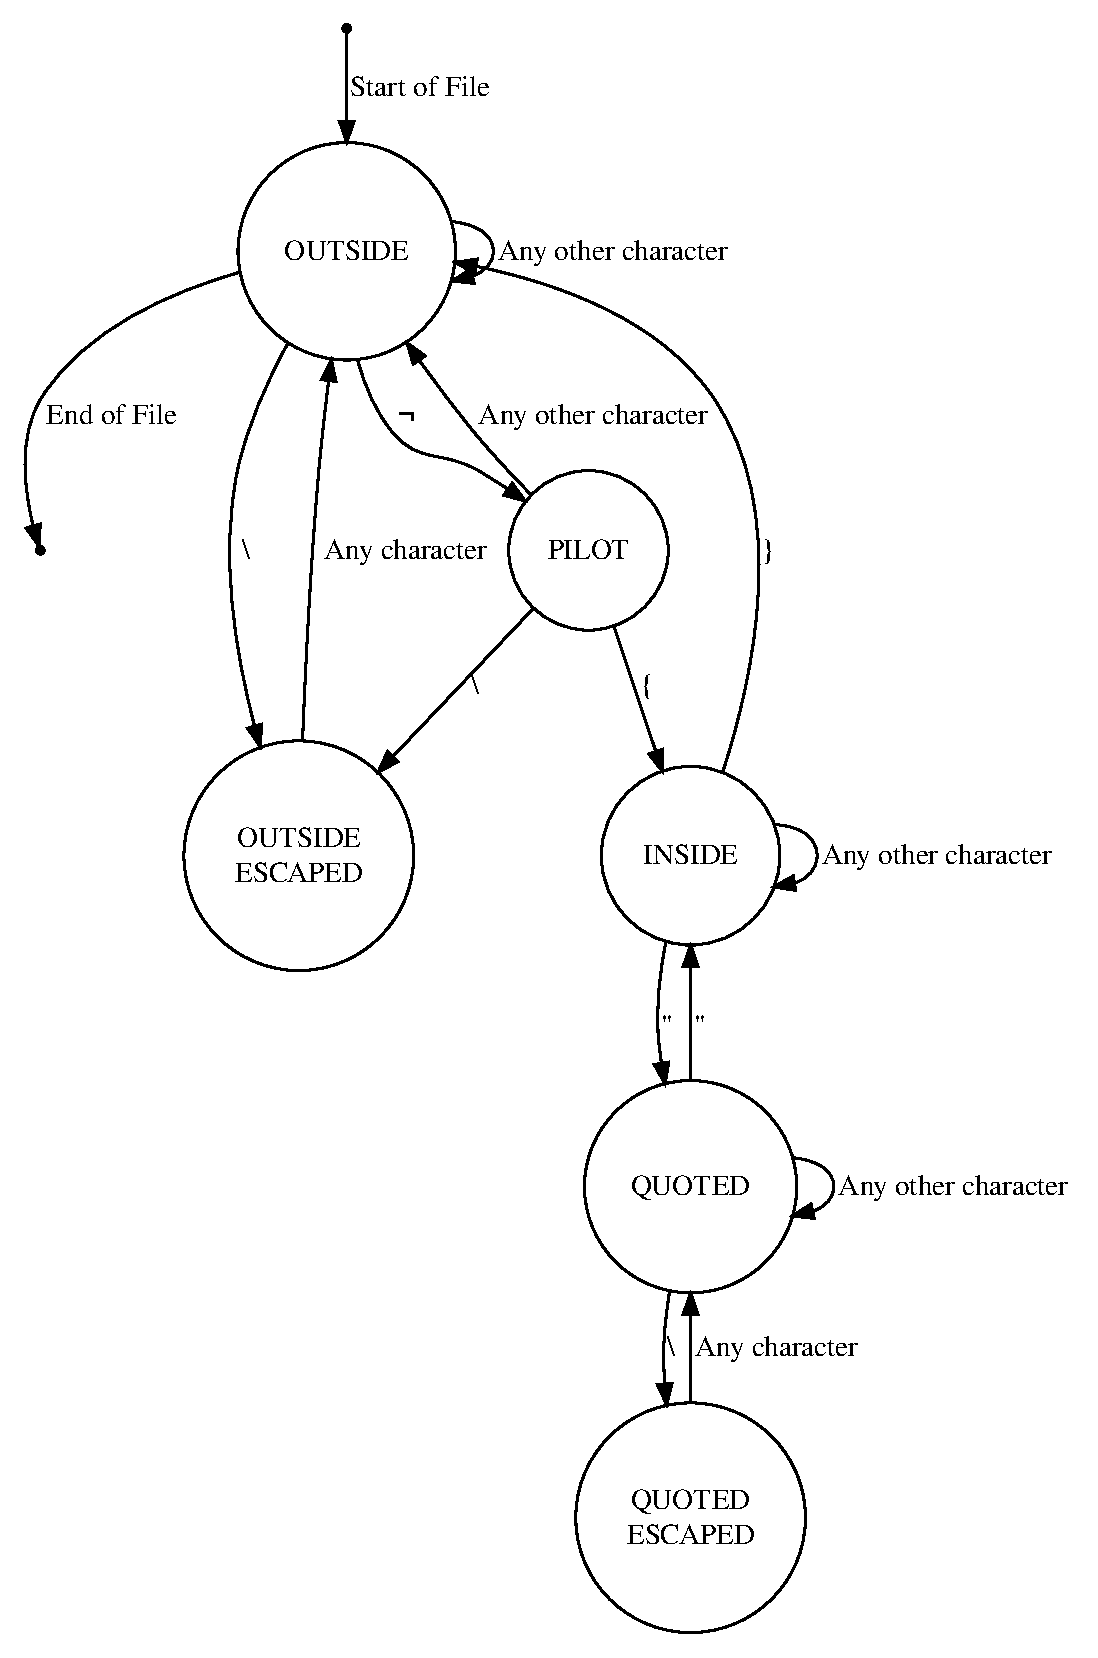
\includegraphics[width=130mm]{Figures/statemachine.eps}
\caption{\label{state machine}Placeholder state machine}
\end{figure}

\subsection*{Nodes and Node Types}
\label{gilt:parser:nodes}

Although an intermediate template document is on one level just a sequence of characters, this is not a very useful abstraction for understanding the intent of the template and converting it to another form. Instead, this parser examines the input document and converts it to a collection of `nodes'. Each node represents some part of the input document. The Nodes have been chosen, wherever possible, to align with the key concepts of template languages. Each node should contain enough information to enable it to be rendered into an equivalent concept in the target template language.

The nodes produced by the parser form a broad-based tree structure. The root of the tree is a sequence of nodes representing the `top level'. This level includes nodes such as text nodes representing boilerplate text and lookup nodes representing a value to be inserted in the output when a template is expanded. Some of these top-level nodes, however, may include other nodes within them. For example, a conditional node requires a discriminator value, which will usually be a lookup node. The action or actions associated with the conditional node might be other nodes such as a text node representing literal text, a block reference node with the name of a block to render, a template inclusion node, and so on.

Every node implements a single Java interface, shown below.

\begin{lstlisting}[backgroundcolor=\color{black!5},escapeinside={(*}{*)},tabsize=2,label={gilt:Node.java},caption={Parser Node interface},captionpos=b]
public interface Node {
	static final String VALUE = "value";

	String getType();
	Map<String,Node> getContent();

	default Node get(String key) { return getContent().get(key); }
	default Node getValue() { return get(VALUE); }
	default String getText() { return null; }
}
\end{lstlisting}

This allows each node to contain a collection of other named nodes, with one given priority as the `value' of this node to simplify code for the common case of boilerplate text and simple lookup or template inclusion nodes. Each node also has a `type' to enable the code in the template generator to decide what to do with the node and how to render it to the destination template language. The template generation code knows nothing about the individual classes which implement this interface, but deal exclusively in the Node interface and its methods.

The various node types produced by the parser have a lot in common. For ease of implementation, some of these similarities have been gathered into an abstract helper class \verb!AbstractNode!. All the implementing classes extend from this class in order to make use of its facilities. The \verb!AbstractNode! class provides an internal data structure to store the inner nodes as well as methods which the individual Node implementations can use to add inner nodes. In addition, the \verb!AbstractNode! class provides methods for diagnostic output which were used when testing the intermediate language parser.

The node types produced by this parser are as follows:

\paragraph{Text node}

A text node represents a block of plain text. This text may be boilerplate text, found between placeholders or at the start or end of the document, or it may be literal text found within the definition of a placeholder. In either case, the intention is the same. When generating a template in the target template language, a text template will be rendered as text. A text node has one internal value, the text itself.

\paragraph{Block Start Node}

A block start node represents the start of a named block. A block start node has one internal value, the name of the block. A block start node is always a top-level node

\paragraph{Block End Node}

A block end node represents the end of a named block. A block end node has one internal value, the name of the block. A block end node is always a top-level node.

\paragraph{Block Reference Node}

A block reference node represents the use of a named block. A block reference node has one internal value, the name of the block. Although a block reference node can be a top-level node, it is more usual to encounter it as the action associated with another node such as a conditional node or a loop node.

\paragraph{Lookup node}

A lookup node represents the fetching of a value from the template context. A lookup node has one mandatory internal value, the name of the value to look up. This node can also contain some optional internal values: a field to access, a method to invoke, and a collection of parameters for that method. In the initial implementation of the intermediate language parser, field and method access are exclusive, so a lookup node can contain a field name, a method name, or neither. Method parameters can only be present if a method name has been specified. The context value name, field name, and method name are all simple text values, but the collection of method parameters can include multiple parameters and those in turn can be literal values or other nodes. The collection of method parameters is represented as an array node (see below).

\paragraph{Template Inclusion Node}

A template inclusion node represents the inclusion of one template by another. The single internal value is a Node representing how to find the name of the template to include. In the initial version of the intermediate language and the parser this internal value can be either a literal text node or a lookup node. More complex configurations such as including a template whose name is given in a file are not supported.

\paragraph{Conditional Node}

A conditional node represents a decision within the template. A conditional node has one mandatory internal value, a node representing the discriminating value. Although the intermediate language allows this to be a literal, that would usually be a pointless exercise, as the result of the conditional expression would always be the same. For most uses this internal value will be a lookup node representing the context value on which to make the decision.

A conditional node can also have a combination of three optional values. If a value was specified using the \verb!is! keyword then that value will be stored as an internal value to be matched. If an action was specified using the \verb!then! keyword then that value will be stored as an action to be performed if the discriminating expression is `true'. If an action was specified using the \verb!else! keyword then that value will be stored as an action to be performed if the discriminating expression is `false'. The initial implementation of the parser does not prevent the declaration of a conditional placeholder with neither a \verb!then! nor an \verb!else! action. If neither are present, then the conditional node will perform no action and produce no output when the destination template is expanded. The nodes representing the actions will usually be block reference nodes, template inclusion nodes, or literal values.

\paragraph{Loop Node}

A loop node represents an iteration placeholder. A loop node has one mandatory internal value, a node representing the collection to be iterated through. While this could potentially be a literal, the initial intermediate language has no syntax to specify multi-value literals, so that is not likely to be a valid type to be iterated in the destination template language. In most cases the node representing the collection will be a lookup node which specifies how to retrieve the collection from the template context. The action to be performed for each element of the collection, specified using the \verb!do! keyword, is theoretically optional, although a loop with no action would generate no output when the destination template is expanded. The node representing this action will usually be a block reference node, a template inclusion node, or a literal value. Two extra internal values are also optional. If a symbol is specified using the \verb!with! keyword it will be stored for use when the destination template is generated. If an element separator is specified using the \verb!separator! it will be also be stored as an internal value. The separator value can be any of the action node types used for \verb!do!, above.

\paragraph{Method Call Node}

A method call node represents a method call placeholder. Although this type of node was supported in the initial intermediate language, and thus the initial parser and generator implementations, it was later subsumed into the lookup node, In the initial implementation it had two mandatory internal values, a lookup node representing the context value on which to invoke the method and a literal value containing the name of the method. As with the method call option of the lookup node, there was also the option to include a collection of parameters. If present, they were stored using an array node.

\paragraph{Array Node}

An array node is an internal node which cannot appear as a top-level node. An array node is created whenever another node needs to contain an unknown number of internal values. Specifically, in the initial implementation of the template language model it is used to contain the list of nodes representing method parameters in both lookup nodes and method call nodes.

\paragraph{Reference Node}

As discussed above, for the intermediate language to express the notion of a current loop element in a way which is independent of the destination template language, it requires a symbolic way to indicate when the current loop element is to be mentioned during template generation. This is the purpose of the reference node. A reference node is produced when a placeholder which starts with the \verb!reference! keyword is parsed. A reference node has one internal value containing the name of the symbol to be referenced. If no symbol name is specified in the reference placeholder, the default value of `this' is used.

\paragraph{}

\subsection*{Character Buffering}
\label{gilt:parser:buffering}

As discussed above, the aim of the intermediate language parser is to convert an incoming template into a sequence of nodes representing the parsed components of the template. Each node typically represents a block of characters from the input template. Each chunk of boilerplate text is represented as a single node, regardless of the length of the chunk. Likewise, each placeholder is represented as a single node with internal values indicating the type of placeholder and the combination of directives and values within it. In both these cases, the content of the node to be constructed is not known until the end is reached. The end of a chunk of boilerplate text is indicated either by the end of the input or by the start of a placeholder. The end of a placeholder is indicated by the terminating \verb!}! character.

The intermediate language parser includes a buffer to collect the text which will ultimately be converted to a node of one sort or another. From the start of a chunk of boilerplate text, or the start of a placeholder, incoming characters are accumulated into a buffer. At the end, the contents of the buffer are converted to a node. Accumulated boilerplate text is directly converted to a text node. Accumulated placeholder text is passed to a separate \verb!PlaceholderParser! object which processes the contents of the buffer according to the grammar of placeholder contents. When the node has been created, the buffer is cleared ready to begin collecting characters for the next node.

Adding text to the buffer normally happens on the `any other character' transitions when the state of the state machine (INSIDE or OUTSIDE) remains the same. Special characters such as placeholder delimiters are not usually added to the buffer, as they serve to indicate the start or end of a node. However, here are a few situations in which special characters are added to the buffer. Any `escaped' characters are added to the buffer, although the escape character (\verb!\!) is not. Quote characters (\verb!"!) in placeholders change the state for the purposes of parsing, but are added to the buffer along with the rest of the placeholder characters. The most complex case is if a `pilot' character (\verb!¬!) is encountered but it is not followed by the \verb!{! which would complete the start of a placeholder (or there is a \verb!{!, but it is escaped). In this case, both the pilot character and the current character need to be added to the buffer. This is the only case in which the parser needs to `undo' a decision while parsing.

\subsection*{Parsing of Placeholders}
\label{gilt:parser:placeholders}

Once the enclosing \verb!¬{! and \verb!}! have been stripped off, each placeholder consists of a sequence of characters which need to be parsed according to the placeholder grammar to determine which specific node or nodes to create. A formal specification for the placeholder grammar is given in \autoref{appendix:bnf initial}. Within a placeholder, unquoted whitespace characters are not significant and are removed as the placeholder contents are parsed. In the following discussion of the parsing process, such whitespace will be ignored. 

As mentioned above, the keywords in the intermediate language have been carefully chosen so that they all have distinct starting letters. The top-level `action' symbols which can start a placeholder, and the node classes which result are shown in the table below. A placeholder that starts with any character not in the table is invalid. A parse error will be produced and parsing will stop.

\begin{table}[ht!]
\fontsize{9}{11}\selectfont
  \begin{center}
    \begin{tabular}{rlll}
      \textbf{Character} & \textbf{Keyword} & \textbf{Description} & \textbf{Node class} \\
      \toprule
      \multicolumn{4}{c}{Top-Level Keywords} \\
      \textbf{i} & \verb!if! & conditional & \verb!IfNode! \\
      \textbf{f} & \verb!foreach! & loop & \verb!LoopNode! \\
      \textbf{s} & \verb!start! & block start & \verb!BlockStartNode! \\
      \textbf{e} & \verb!end! & block end & \verb!BlockEndNode! \\
      \textbf{b} & \verb!block! & block reference & \verb!BlockNode! \\
      \textbf{t} & \verb!template! & template inclusion & \verb!TemplateNode! \\
      \textbf{l} & \verb!lookup! & value lookup & \verb!LookupNode! \\
      \textbf{r} & \verb!reference! & symbol reference & \verb!ReferenceNode! \\
      \textbf{"} & & \emph{quoted literal} & \verb!TextNode! \\
      \hline
      \multicolumn{4}{c}{Context-Specific Keywords} \\
      \textbf{d} & \verb!do! & loop body & \emph{various} \\
      \textbf{e} & \verb!else! & action if false & \emph{various} \\
      \textbf{i} & \verb!is! & conditional match value & \verb!TextNode! \\
      \textbf{f} & \verb!field! & lookup field name & \verb!TextNode! \\
      \textbf{m} & \verb!method! & lookup method name & \verb!TextNode! \\
      \textbf{p} & \verb!parameter! & method parameter & \emph{various} \\
      \textbf{s} & \verb!separator! & loop separator & \emph{various} \\
      \textbf{t} & \verb!then! & action if true & \emph{various} \\
      \textbf{w} & \verb!with! & loop variable name & \verb!TextNode! \\
    \end{tabular}
  \end{center}
\caption{Keyword Initial Characters}
\label{gilt:table:initial characters}
\end{table}

The placeholder parser examines the initial character of the placeholder and calls an appropriate parse method for each placeholder type. This parse method is responsible for parsing the rest of the placeholder and returning a \verb!Node! object representing it. Each method (except for quoted literals which effectively have a single character keyword) begins with a call to a method \verb!expect! which is given the full text of the keyword, for example by calling \verb!expect("lookup")!. This method steps through the incoming character stream checking that the specified characters are present. If the keyword ends prematurely, or contains an unexpected character, then a parse error will be produced and parsing will stop. Once the initial keyword has been verified, the code for the parse method depends on the specific nature of that type of placeholder. The sequence of methods called to parse the remainder of the placeholder follow the grammar.

As a simple example, a block start placeholder is defined in the grammar specification as the keyword \verb!start! followed by a literal, so in the method for a block start, the keyword is verified, then the \verb!literal! method is called to parse a literal value. All the parse methods return a \verb!Node! object, including ones which cannot be used at the top-level of a placeholder, so in this case calling the \verb!literal! method results in a \verb!TextNode! object representing the literal text. As the literal value is the only extra node in this case, as soon as the \verb!TextNode! object is returned from the \verb!literal! method it is used as the value when constructing a new \verb!BlockStartNode! which is then returned from the parse method.

Block end and block reference placeholders also require a single literal value following the initial keyword, so the structure of their parse methods is similar to the block start method. Other parse methods are more complex, however, as they have options which need to be correctly recognised and processed. In such cases the process is similar to the process for the `action' symbol used at the top-level of a placeholder. The next character of the input stream is examined and checked against a list of valid options. If a valid initial character is encountered, then parsing is handed off to the appropriate parse method.

For example, the \verb!conditional! method is used to parse placeholders which start with \verb!if!. The placeholder grammar indicates that the next item must be a `value', so the \verb!value! method is called to return a \verb!Node! object representing that value. After the value, there are several optional items. The next item can be either \verb!is!, \verb!then!, \verb!else!, or nothing at all. A Node variable is prepared in advance for each option and set to \verb!null!, indicating that the particular option has not been provided. If the placeholder ends at this point, then the resulting \verb!IfNode! object will have no internal values for the value to match, the action on true, or the action on false. If the next character in the placeholder is one of \verb!i!, \verb!t!, or \verb!e!, then the process continues with an appropriate parse method, which follows the same pattern as all the parse methods. Call \verb!expect! to verify the full keyword, then combine the mandatory and optional following values into a \verb!Node! object which is then returned. Each returned value is placed into the variable prepared for that purpose. When the placeholder ends, the collected variables are combined into an \verb!IfNode! which is returned from the method.

The \verb!Node! objects resulting from top-level placeholders are then added to the sequence of nodes which represent the template as a whole, alongside any \verb!TextNode! objects resulting from boilerplate text. This sequence of nodes is what is passed to the template generator for rendering into a destination template.

The parsing approach described above correctly implements the placeholder grammar, but that does not mean that all possible combinations of nodes and sub-nodes are useful.  For example, as can be seen from the table of initial characters, a placeholder which starts with a double-quote character represents literal text and results in the creation of a \verb!TextNode! object. While this is legitimate according to the placeholder grammar, it is generally not very useful, as the resulting node is indistinguishable to the generator from a section of boilerplate equivalent to the quoted text. Likewise, an \verb!ifNode! with none of the optional values, although valid, represents a template action that examines a value but does nothing with it, so it will not result in any output when the generated destination template is expanded. Depending on the syntax and semantics of the different destination template languages, such pointless constructs may not even be able to generate valid templates.

\section*{The Template Generator}
\label{gilt:generator}

The job of the template generator is to take a template expressed in the intermediate language and convert it, where possible, to a similarly-functioning template in a destination template language. Conversion is not always possible, however. The intermediate language is designed to support a set of common template language features but these are not supported in all template languages.

There is only one intermediate language, so the template generator creates an instance of the intermediate language parser which it uses to parse a supplied intermediate template to produce a sequence of \verb!Node! objects representing the various chunks of boilerplate text and placeholders from the original template. To produce a destination template, the template generator passes the parsed sequence of Nodes to a template language driver which understands how to render each type of Node into the syntax and grammar of the destination template language.

\subsection*{Template Storage and the Tract class}
\label{gilt:tract}

Different template engines have different requirements for template storage. Some template engines expect a template to be provided as a text string in memory, some require that every template exists in a file, sometimes with a specific filename, location or file type. The Template generator cannot know about the vagaries of every possible template engine, so an abstraction is required to isolate the generation process from such details.

The template generator treats every template as an object which implements the \verb!Tract! interface. The Tract interface provides a small set of methods to access the content (in this case the text of the template) and a collection of name/value properties. In this use of the \verb!Tract! concept, the properties depend on the requirements of the specific template engine. Some template engines will not need properties in addition to the text of the template, while others may require details of, for example, how and where the template should be stored.

When Tract objects need to be retrieved from storage, there is another abstraction \verb!TractSource!. \verb!TractSource! is also an interface which provides a method to retrieve a \verb!Tract! by name, and also some general purpose methods to enquire about the \verb!TractSource! itself, such as whether it is empty or where it is located. By default, a \verb!TractSource! is read-only, but a further interface \verb!WritableTractSource! extends this to support placing a \verb!Tract! into the store as well as removing a stored \verb!Tract! or clearing the store.

\verb!TractSource! (and \verb!WritableTractSource!) implementations can be created to represent the details of how and where templates are stored. The template generator can use the \verb!TractSource! methods on a provided store object with no knowledge of the underlying implementation.

\subsection*{Drivers and Dynamic Loading}
\label{gilt:plugins}

Using the same justification as the design of the dynamic loading mechanism for template engine drivers during template engine comparison (as described in \autoref{comp:plugins:dynamic}), each template language driver is implemented as a separate `plugin'. When generating templates for a particular template language, the plugin is specified as a command-line parameter which adds the plugin classes to the Java classpath of the running generator.

The template generator refers to a class named \verb!plugin.DriverFactory! which serves the same purpose as the class \verb!plugin.EngineFactory! described in \autoref{comp:plugins:dynamic}. All implementations of \verb!plugin.DriverFactory! implement a Java interface which specifies the methods it must implement. In a similar pattern to \verb!plugin.EngineFactory!, the interface implemented by template language drivers contains just two methods, as shown below.

\begin{lstlisting}[backgroundcolor=\color{black!5},escapeinside={(*}{*)},tabsize=2,label={gilt:DriverFactory.java},caption={Parser DriverFactory interface},captionpos=b]
package shared;
import java.io.IOException;
import com.efsol.templates.TemplateDriver;

public interface DriverFactory {
	TemplateDriver create() throws IOException;
	String getName();
}
\end{lstlisting}

As an example, the code for this class in the \emph{Trimou} plugin is shown below.

\begin{lstlisting}[backgroundcolor=\color{black!5},escapeinside={(*}{*)},tabsize=2,label={gilt:trimou:DriverFactory.java},caption={Trimou DriverFactory interface},captionpos=b]
package plugin;
import java.io.IOException;
import com.efsol.templates.TemplateDriver;

public class DriverFactory implements shared.DriverFactory {
    @Override
    public TemplateDriver create() throws IOException {
        return new TrimouTemplateDriver();
    }

    @Override
    public String getName() {
        return "trimou";
    }
}
\end{lstlisting}

\section*{Potential Improvements to the Intermediate Language}
\label{gilt:language plus}

\paragraph{Redefinable Delimiters}
The choice of characters to delimit the start and end of placeholders was largely arbitrary, based on locating a character sequence not significant in the available template languages and not common in content for common document types. This choice raises some issues, however. One problem is that the initial `pilot' character \verb!¬! is not available on all keyboards. Although more common, the \verb!{! and \verb!}! can also be difficult to enter on a range of keyboard layouts \citep{Erz2023a}. It is usually possible to enter these characters if needed, but the methods can be clumsy, such as entering a multi-digit character code, or copying the character from elsewhere and pasting it into the text. This can make working with intermediate templates far from the intended comfortable experience. Another problem is that if a desired target document type \emph{does} use these characters, then frequent escaping will be required, with any failure to escape these characters leading to errors and invalid templates.

Without knowing every possible future keyboard layout or document type it is impossible to determine a `perfect' set of delimiter characters. To address these issues would require some way to redefine the characters to be used to delimit placeholders, allowing characters to be chosen which are both easy to type and minimise conflicts with document content. There are several ways to achieve this including: requiring users to change and re-compile the parser code itself; command-line parameters, configuration files, or other run-time parser settings; and configuration overrides associated with either individual templates or all templates retrieved from a particular template source location.

Global settings such as code-editing or configuration files persist between template generation runs and tend to have a relatively long life, so these approaches might be suitable for configurations related to hardware such as keyboard layouts. Such long-term settings would be less suitable for adapting to specific document formats, however. These might be better served by configuration overrides associated with individual or groups of templates.

Improving the intermediate template parser to support redefinable delimiter characters would require code changes to remove the dependency on literal delimiter characters in the code and to accept redefinitions from a range of sources. The initial implementation of the template parser and generator does not have any external configurations, so any external redefinition of these characters would require extra code to support that. One of the aims of the development was to create a system which is portable for many uses and situations, so relying on configuration mechanisms specific to particular operating systems or file structures would not be appropriate. An initial solution for persistent configurations which adapt the system to the local environment is to use command-line parameters. These are supported, in one form or another, by all common systems and can be made more-or-less persistent by including them in whatever script, shortcut, or desktop icon is used to launch the template generator.

The possibilities for setting overrides which apply just to one template or to a specific group of templates are just as varied. The same command-line options as for local environment settings can also be used for this task, but that is likely to lead to a proliferation of scripts and launchers and the concomitant increase in the risk of mistakes. Anther option includes some form of configuration file placed in the same location as some of the intermediate templates or with the same name as some of the intermediate templates. The system would then be able to look in this configuration file before attempting to process an intermediate template. While this system is plausible, it ties the configurations not just to the intermediate template contents, but to its name or location. If either of these are changed, then any associated configuration files would need to be changed to keep them in step. This approach also potentially slows down template processing, as the system would need to check for the existence of any associated configuration overrides before parsing, even if no such configuration overrides exist for that particular template. Similar problems would be faced by solutions involving a single centralised configuration explaining which configurations to use under which circumstances. To avoid such accidental coupling, it seems logical to place any configuration overrides which affect the processing of a template inside the template itself. With this approach, templates can be moved or renamed with no impact.

The challenge with including configurations within a file is to reliably distinguish them from the rest of the file's contents. For any configurations which do not affect the characters used as delimiters, this would be a relatively simple operation. Just introduce a new type of placeholder directive which allows the definition of a configuration, then include such directives before any other placeholders or directives which make use of the new configuration. This approach is arguably possible even for configurations which change the delimiter characters, but this would result in a template file containing both old and new delimiters and impose constraints on the order of the parsing process.

An alternative is to use a completely different syntax to indicate configuration settings. There is precedent for including such `header' text in a wide range of files, from the collection of name-value pairs found at the start of HTTP messages and emails, to delimited blocks of JSON or YAML data. The challenge is to unambiguously indicate the presence in such a header without assuming anything about the potential content of the file. HTTP and email documents do this by asserting that there will always be such a header, even if it is empty. The working assumption for this intermediate language is that such per-file overrides will be relatively rare, used only in the cases where the neither the default configurations nor any local command-line overrides are suitable for a particular file's contents. The overhead of always requiring a header seems too much for such rare cases, so a delimited approach seems more appropriate.

Typical JSON and YAML headers use repeated multi-character delimiters such as \verb!---! on a line of their own at the start and end of the header block, and also require the header block to be the very first content in the file. This enables a parser to quickly determine the presence or absence of the header block by analysing the first few characters in the file. There is, of course, always the risk that legitimate file contents might also start with this character sequence, but experience has shown that this is extremely rare. Even for cases of such a clash, the header block is only parsed once so placing an header block, which can be empty, at the start of a template would then allow the header prefix to be used within the template. An alternative approach would be to use the command-line configuration discussed above to define an alternative starting and ending sequence for such a configuration header.

This situation does not need many configuration options, so the structural overhead of JSON or YAML parsing seems unnecessary. A simpler name/value list, similar to HTTP and email headers would appear to be sufficient. An example intermediate template with a header block overriding the intermediate language delimiters might therefore look like:

\begin{lstlisting}[backgroundcolor=\color{black!5},escapeinside={(*}{*)},label={gilt:delimiter override},caption={Potential delimiter override syntax},captionpos=b]
---
delimiter start: %<
delimiter end: >
---
%<foreach lookup "prices" do template "price" separator ",">
\end{lstlisting}

Note that while the choice of starting delimiter can be anything which does not conflict with the boilerplate content, the choice of ending delimiter is limited to a single character which cannot appear unquoted within a placeholder or other directive.

\paragraph{Nested Blocks and Name Repetition}

In the intermediate language, named blocks are used to indicate sections of boilerplate and intermediate template markup which are used with control structures such as conditional and iteration directives. The design of the initial language allows these blocks to be nested with other named blocks, and in order to correctly detect and report on incorrect nesting or blocks without an end directive, both the start and end directive for each block must contain the same name. This approach is also used in HTML and XML markup \citep{Bray2008}. However, this requirement for the repetition of the name potentially increases the fragility of the language. Some other forms of markup chose only to indicate the name or type of a block at the start, and use a generic end for all blocks.

Although repeating the block name at the end has a range of benefits, such as making it slightly easier to find the other end of a block, or to remind a reader when a block is too long to take in all at once, the primary benefit of the repeated names is for error detection and reporting in the case of malformed nested blocks. While nested blocks can make more sense to some readers, as they can more closely mirror the expected structure of the generated template in some template languages, they are not strictly necessary for the template generation process to work correctly. All named blocks exist in the same namespace and will be located and used wherever they are positioned in a template.

If nesting of templates were to be prohibited, then the repetition of the name would no longer be so useful for error detection and reporting, and a more generic \verb!end! directive could be used.

\paragraph{Null Values and The Potentially Redundant Call Directive}

In the initial design for the intermediate language, code execution through method calls was envisaged as a separate concept to looking up a value from the supplied template context. Method calls have their own directive \verb!call!, distinct from the \verb!lookup! or \verb!template! directives allowed in value placeholders. Following use of the intermediate language, however, it became apparent that method calls were usually used as just a special case of value placeholder, especially when value placeholder processing was enhanced to allow field, method, and JavaBean access from context values.

If the intermediate language were being designed purely as a template language in its own right, this would not be an issue, the syntax for specifying method calls could be merged with that for value placeholders with no major impact. The main purpose of the intermediate language, however, is as a representation which can be automatically transformed into other template languages. Some of those other template languages do separate the two concepts. In the \emph{JSP} template language, for example, these two concepts even have different delimiters to distinguish them within templates \citep{Oracle2000}. The distinction exists because some methods are declared as not returning a value, so there will be nothing to put into the output document as a result of the method execution. Some template engines can cope with a placeholder which does not provide a value, treat it as if the placeholder had provided an empty string, and so render nothing into the output document. Other template engines will either fail to process the template, or insert some error message or other unwanted text into the output document. Such template engines, if they support method calls at all, usually require a separate syntax to indicate that the method is not expected to return a value and therefore does not provide any text to include in the output document.

At the time at which the intermediate template is processed to generate the `real' templates, nothing is known about run-time details such as whether a method call will return a value, or whether a context value or field will be null. Arguably the intermediate language should provide a way for template authors, who may know more about what is supposed to happen when the target template is expanded, to indicate in the intermediate language markup whether a method call is expected to return a value, so that the generation process can select appropriate syntax when generating a template. In the initial design for the intermediate language, the separate `call' directive provides a way to indicate this, but the behaviour is implicit rather than explicit and may not be obvious to a template author who is not familiar with how the generation process works.

A better solution to this issue would be to merge the value placeholder and method call syntax, but allow optional explicit markup on any placeholder to indicate that it is not expected to provide a value for the output. A potential syntax for this might look like:

\begin{lstlisting}[backgroundcolor=\color{black!5},escapeinside={(*}{*)},label={gilt:lookup method call},caption={Potential merged lookup method call syntax},captionpos=b]
(*¬*){lookup "product" method "price" parameter "GBP" void}
\end{lstlisting}

where the keyword \verb!void! indicates that either the method returns no value, or that the value should be discarded and not added to the output document.

\paragraph{Explicit Types for Context Values and Method Parameters}

Most template languages, and the template engines which implement them, are `weakly typed' - they have only a loose notion of data types. In such languages, a data item is required to have a value which can be represented as text, but the actual type of the value is largely unimportant. This becomes a little more complex when the template language supports features such as field access, list element iteration, or method calls. These actions require an object of a type which supports such operations, but this is usually only checked when the action is executed during template expansion. An attempt to, for example, access a named field of an object which does not have a publicly available field of that name will result in some form of error or warning when the template is expanded. This may, in turn result in no value appearing for that value, an error message of some sort appearing in the output document, or the template failing to expand at all. Although they are less common, with only one example in the cohort of template engines under consideration for this research, some template languages are `strongly typed' \citep{Fokkinga1981} \citep{Madsen1990}. This kind of template language requires that all context variables and other data values have an explicit associated type. Any attempt to use a value with an incorrect type can then be caught at the start of template expansion.

The initial version of the intermediate language does not support typed values, nor any way to refer to non-core classes, so for strongly-typed template languages it is assumed that all values are of type String. This obviously works only if the values are actually of type String, and will generate an incorrect output template whenever different types are required. To address this issue, and enable the template generator to produce correct templates for strongly-typed template languages the intermediate language would need enhancement to allow specification of value types. These type specifications would not be required or used when generating templates for weakly typed template languages. For practicality, it would seem reasonable to make such annotations optional, only required when the value datatype is other than String. Potential syntax for this might look like:

\begin{lstlisting}[backgroundcolor=\color{black!5},escapeinside={(*}{*)},label={gilt:variable types},caption={Potential value type syntax},captionpos=b]
(*¬*){lookup "stocklevel" type "java.lang.Integer"}
\end{lstlisting}

This indicates that the context value stored with the name `stocklevel' is of type `java.lang.Integer'. All types starting with `java.lang.' (indicating that they are part of the `java.lang' package) are built-in types in Java and do not need an `import' directive. Where no package is specified, it is assumed to be `java.lang', so this type could also have been written as `Integer'.

A similar approach would also be suitable for method calls, as shown below.

\begin{lstlisting}[backgroundcolor=\color{black!5},escapeinside={(*}{*)},label={gilt:parameter types},caption={Potential type syntax for method calls},captionpos=b]
(*¬*){lookup "product" type "com.shirtshop.Sku" method "price" parameter "GBP"}
\end{lstlisting}

In this case the context value stored with the name `product' is defined to be of type \verb!com.shirtshop.Sku!. As the type name does not start with \verb!java.lang!, it indicates an external class which would need an \verb!import! declaration in a strongly-typed template language such as \emph{JTE}. The template engine which processes such a template would then be able to determine whether the `product' object exposes a method named `price' prior to attempting to call the method.

\paragraph{Constants and Variables}

In a general-purpose programming language it is very common to give names to intermediate values. This both assists with the readability of the code and enables these values to be re-used without the need for recalculation. Template languages often borrow features from general-purpose programming languages so it should come as no surprise that some template languages also have this feature. Most general-purpose programming languages make the distinction between a `constant', whose value is defined to remain the same for the whole execution of a program, and a `variable' which may be later redefined to a different value. These concepts are not universally applied, however. Some programming languages, such as \emph{Haskell}, treat all values as immutable and so do not really have the concept of variables \citep{Marlow2010}, while others, such as \emph{Lisp} treat everything as changeable, even the program code.

A template language is not the same as a general-purpose programming language, however, as it lacks the concept of sequential execution which characterises most general-purpose programming languages. Conceptually a template is all evaluated at once. This makes the key characteristic of variables - that they may change over time - a difficult concept to determine. Template engines address this in a variety of ways. Some, typically the ones which compile a template into a program, method, or subroutine in a general-purpose programming language as a first step in expanding it, embody the assumption that a template is evaluated top-to-bottom. In such a model, variables make sense and the same variable name can be redefined to take different values as the template is processed. Others, typically ones in which a template is parsed into a tree or other internal representation as a first step in expanding it, may evaluate placeholders and other template expressions in an arbitrary order. In such a model, variable life-cycles do not make sense, so where such template languages support named intermediate values they are usually immutable and more like constants than variables, even if the syntax implies variability.

It would be possible for the intermediate language to support named intermediate values to be rendered as variables in the target template language, but the semantics of the template variables would depend entirely on the template engine which eventually evaluates the generated template. It would also be possible for the intermediate language to support constants or variables which are not passed through to be rendered as variables in the target template language but instead used by the intermediate language itself during the generation of templates. The main advantage of this would be similar to the approach of naming blocks within the template - to increase readability and to enable re-use of common template expressions without the need to redefine them multiple times. In this sense such a definition would be more akin to a `macro' than a more traditional constant or variable.

An potential syntax for named values might look like:

\begin{lstlisting}[backgroundcolor=\color{black!5},escapeinside={(*}{*)},label={gilt:variables},caption={Potential variable definition syntax},captionpos=b]
(*¬*){define "cost" as lookup "product" method "price" parameter "GBP"}
\end{lstlisting}

In this case a value named `cost' is defined as the result of calling the method `price' with a single String parameter `GBP' on the context object with the name `product'. The defined value can then be referenced in a regular \verb!lookup! directive, as if it is stored in the template context. When generating a template in a language which supports such named values, this can be rendered using the appropriate syntax. When generating a template in a language which does not support named values, the template generator will fall back to rendering the complete value expression wherever it is used, in the style of a macro.

\paragraph{Non-literal Parameters to Methods}

The initial implementation of the intermediate language has inconsistent support for indirect values. For example, it supports the use of a context value as the name for a template to be included. However, initial support for method calls was based on calling \emph{JavaBeans} or other methods without parameters. Method parameters were added later in development and are always assumed to be literal values. While literal parameters may make sense for some specific cases, in the general case it is likely that some methods will need parameters which are different for different uses of the template and should therefore be stored in, and retrieved from, the template context. A more consistent approach to method parameters would allow for context values as parameters and possibly even indirect context values such as using the context value as the name of another context value. A potential syntax for such parameters might look like:

\begin{lstlisting}[backgroundcolor=\color{black!5},escapeinside={(*}{*)},label={gilt:lookup params},caption={Potential non-literal parameter syntax},captionpos=b]
(*¬*){lookup "product" type "com.shirtshop.Sku" method "price" parameter lookup "currency"}
\end{lstlisting}

This approach is not without its own issues, however. If the syntax were to be fully extended to also support method calls as a way to provide method parameters, there is the potential for confusion as to which method `owns' each parameter. In most general-purpose programming languages, this is addressed by the use of parentheses or other delimiters to group the parameters for a particular method call. So far, the design of the intermediate language has been suitable for deterministic parsing without the need for such delimiters, and adding them could add unwanted complexity to the parser and thus the template generation process. A similar problem could also occur with field access specifiers.

Support in destination template languages for any kind of method calls is not universal (see \autoref{fs:table:features}), and support for complex features, such as the use of the results of method calls as method parameters, is rarer still. If the intermediate language were to forbid method calls and field access in method parameters for the sake of faster and more deterministic parsing it is not clear how much this might impact real usage. If the intermediate language were to support context values as parameters, then in many cases the result of the subsidiary method call could be pre-calculated and placed into the template context or set as a template `variable' as described above.

\paragraph{Direct Access to Collection Elements}

As well as simple values, field access, and method calls, some template languages, such as \emph{Velocity}, support additional options on lookup placeholders. One such additional option is the ability to access indexed elements from arrays and other ordered collections. The \emph{Velocity} template fragment shown below represents accessing the first element from an ordered collection or array stored in the template context with the name `releases'.

\begin{lstlisting}[backgroundcolor=\color{black!5},escapeinside={(*}{*)},label={gilt:arrays},caption={Potential collection element syntax},captionpos=b]
$releases[0]
\end{lstlisting}

Internally within the \emph{Velocity} template engine this is translated to an appropriate way to access the element from the value. If the value is an array, then the Java array element syntax is used. If the value implements the \verb!java.util.List! interface, then a \verb!get()! method is called on the object passing in an integer to indicate the position in the list. This same syntax is also used for accessing values from an associative array. If the value implements the \verb!java.util.Map! interface, a similar \verb!get()! method is used to retrieve the value associated with a specified key.

The initial implementation of the intermediate language does not support this feature. Although the associative array aspect of this functionality can be emulated using the lookup method call syntax, all keys must be text strings, as there is no way to specify a literal integer value. As with so many features found in specific template languages, it is not clear how often this feature is used in live templates, or whether there is any way to effectively emulate it in template languages which do not support this feature.

\paragraph{Abbreviated Keywords}

During development of the intermediate template language parser there was a discussion about whether to also allow abbreviated or misspelled as well as full keywords. They all have unique initial letters so there would be no ambiguity. This was a technique used in many early implementations of the BASIC programming language \citep{Kurtz1978}, and using just the initial letter of each keyword could considerably reduce the amount of typing for template authors and the size of the intermediate templates. It would not, of course, have any effect on the size of the generated templates. The disadvantages of such an approach would be the potential loss of readability of templates expressed in this language and the need for whitespace or other delimiters to indicate the end of a keyword. This feature is still under consideration, and the initial implementation of the template generator requires full keywords.

\section*{Template Language Drivers}
\label{gilt:drivers}

The aim of the design of the intermediate language is that, after parsing the intermediate template, the resulting data structure contains all the information required to generate an equivalent template in each of the supported template languages. Subject, of course, to the capabilities of the individual template languages. In order to generate the destination templates, however, a mapping is required between the collection of symbolic language nodes held in the data structure, and the textual expression in a particular target template language. For this research, this mapping has been defined in the form of a range of software \emph{drivers}, written in Java. A separate driver has been created for each of the template engines in the cohort. All the template language drivers implement the same Java interface definition, which provides methods to render specific node types from the symbolic model.

\subsection*{Driver Interface and Shared Code}

In conjunction with the initial intermediate language and its parser, a Java interface was defined to provide a set of methods which all template language drivers must implement. The code for the interface is given below.

\begin{lstlisting}[backgroundcolor=\color{black!5},escapeinside={(*}{*)},tabsize=2,label={gilt:interface},caption={TemplateDriver interface},captionpos=b]
public interface TemplateDriver {
	void init(Map<String, Node[]> blocks, WritableTractSource templates);
	String renderNodeArray(Node[] nodes) throws IOException;

	void renderIncludeNode(String templateName) throws IOException;
	void renderBlockReferenceNode(String blockName) throws IOException;
	void renderIfNode(Node key, Node match, Node iftrue, Node iffalse) throws IOException;
	void renderLoopNode(Node target, Node with, Node body, Node sep) throws IOException;
	void renderTextNode(String text) throws IOException;
	void renderLookupNode(Node target, Node field, Node method, Node parameters) throws IOException;
	void renderMethodCallNode(Node target, Node method, Node[] parameters) throws IOException;
	void renderReferenceNode(Node symbol) throws IOException;

	String quote(String text);
}
\end{lstlisting}

In this interface there are three groups of methods. 

The first group consists of methods relating to the whole template generation process.

The \verb!init! method begins the generation process for a new output template. The parameters are a Map of nodes representing the named blocks from the intermediate template and a `place' where templates are stored. The `place' is a virtual location which provides a basic set of operations and can be implemented in different ways, such as a file store, an in-memory store, or even a remote store in a database or server if required.

The first parameter to this method is used during template generation whenever a control structure in the intermediate template refers to a named block. The contents of the block can be fetched from the supplied Map by name as an array of parse nodes and rendered in whatever manner and to whatever location the particular template language driver requires. The second parameter will be used for two situations. The first is if a `template' directive is encountered but the destination language does not support template inclusion. In this case, the template generator will need to render the contents of the included template directly into the output template. The second situation in which the template location will be needed is if the destination template language requires the generation of multiple template files rather than including the block contents in-line in the main template. This location is where generated sub-templates will be placed.

The \verb!renderNodeArray! method is used when rendering either a whole template or a sub-template such as a named block. This method is the main entry point into the driver from the template generator code. This is a separate method from the rest of the `render' methods as, depending on the destination template language and whether it is a `top level' template, the result may be included in the generated template, or it may be stored to the template `place' for direct use or for later inclusion when another template is expanded. The \verb!renderNodeArray! method returns the result as a text string which can then be stored or included as required.

The second group of methods are the core methods of the template language driver for each different template language. Each of these methods handles one of the types of nodes produced during parsing and allows the driver to render that type of node in an appropriate manner for that template language. The method names largely follow the node names and the syntax of the intermediate template language.

The \verb!renderIncludeNode! method allows the template language driver to adapt to the destination syntax for template inclusion and is triggered by the presence of a parse node resulting from a \verb!template! directive.

The \verb!renderBlockReferenceNode! method allows the template language driver to adapt to the destination syntax for sub-templates and is triggered by the presence of a parse node resulting from a \verb!block! directive.

The \verb!renderIfNode! method allows the template language driver to adapt to the destination syntax for conditional control structures and is triggered by the presence of a parse node resulting from an \verb!if! directive.

The \verb!renderLoopNode! method allows the template language driver to adapt to the destination syntax for loop control structures and is triggered by the presence of a parse node resulting from a \verb!loop! directive.

The \verb!renderTextNode! method is triggered by the presence of a parse node resulting from boilerplate text. Note that the parsing process also produces text nodes for literal text within a placeholder but these are handled within the render method for the appropriate placeholder directive.

The \verb!renderLookupNode! method allows the template language driver to adapt to the destination syntax for context value access and is triggered by the presence of a parse node resulting from a \verb!lookup! directive.

The final group of methods enable drivers to adapt to different situations during the processing of nodes.

The \verb!quote! method allows the template language driver to generate quoted and/or escaped text according to the rules for the destination template language.

\subsection*{Commonalities Between Template Languages}

While it would be possible to create a template language driver completely from scratch, based solely on the \verb!TemplateDriver! interface, the resulting code would likely have a lot of similarities to other drivers. This is for three main reasons. The first reason is that there is always a certain amount of general processing which will be needed in all implementations. For example, the code to step through the nodes in an array during processing of the \verb!renderNodeArray! method is very likely to be the same for most, if not all, template language driver implementations. The second reason is that, even in areas where template languages differ, they are not entirely distinct from each other. Some template languages will have similar syntax to others for some operations, or the structure of their syntax will be similar enough that portions of the code to generate the resulting template will be the same. For example in this cohort of template engines, \emph{Handlebars}, \emph{Hapax}, \emph{Jangod}, \emph{Mustachej}, \emph{Pebble}, and \emph{Trimou} all use the same basic syntax for context value placeholders. In this case, the code for value placeholders in all these different driver implementations will probably be functionally identical. A third reason for similarity of code is that the intermediate language is capable of expressing some relatively complex template directives and expressions which only a few template languages support. In these situations, the code for most of the template drivers will consist of an error message indicating that the destination template language cannot support the required construct. If most template languages do not support a particular combination of features, then they could all make use of the same default implementation which produces such an error message.

In cases where there is some similarity between template languages, it can make sense to share code. In the initial implementation of the template generator, all the template language drivers share a base implementation of the \verb!TemplateDriver! interface named \verb!CommonTemplateDriver!. This class defines a default implementation for all of the `render' methods as well as a selection of helper methods to perform operations common to several template language driver implementations.

One of the key methods provided by this class is \verb!renderNode! which examines a supplied node and calls whichever of the other `render' methods is appropriate. This method understands the structure of each of the node types and is able to recognise each node by its `type' field and extract their options and parameters and construct a correct call to one of the specific method to render the node. This method will issue a template generation error if an unknown node type is encountered, but this should never happen unless the parser code is altered without corresponding changes to \verb!CommonTemplateDriver!. In addition to this basic functionality, the \verb!renderNode! method, along with most methods in the \verb!CommonTemplateDriver! class, provides switchable diagnostics to assist a driver author in verifying and debugging driver behaviour.

Some method implementations will be similar for almost all template language drivers. An example of this is the \verb!renderTextNode! method. All the template languages in this cohort render boilerplate text as-is, so the default implementation is very simple - it just adds the supplied text to the output template. There is a slight complication with this method, though. the specification of the initial intermediate language allows any characters which do not introduce an intermediate language placeholder in the boilerplate text. There is a chance, therefore, that boilerplate text may conflict with the placeholder syntax of the destination template language. In such cases, individual drivers can override this method to apply language-specific escaping rules to the supplied text before passing it on to the default method for rendering.

In addition to these key rendering methods, the \verb!CommonTemplateDriver! class also provides a range of overridable methods for common functions such as quoting or escaping text, or appending characters to the generated text in a variety of situations. For example, some template languages require the names of context values included templates to be quoted while others do not. Likewise, some template languages support literal text in place of context values, but these need to be quoted, and perhaps in a different way to template or context value names. The parsed node list resulting from parsing an intermediate template in the intermediate language contains a range of types of nodes including the various kinds of template directives and boilerplate text found outside placeholders. The code to determine when and how to quote or escape the textual values of these nodes could end up repeated in many drivers, so helper methods are provided which deal with common cases. The aim is to provide enough support that drivers only need to include code which is specific to that particular template language.

In the initial implementation of the template generator there is still work to be done in minimising the code requirements for each driver. There are areas where functionally identical code is included in all template drivers. For example, consider the implementation of the \verb!renderBlockReferenceNode! method from the \emph{Velocity} driver shown in \autoref{renderBlockReferenceNode}. This implementation contains no code specific to the \emph{Velocity} template language, and similar implementations are found in the drivers for other template languages. This code should therefore be moved to somewhere accessible to all drivers. Examining the template languages in the cohort under consideration, it appears that most use some form of in-line representation for code blocks, so this implementation is also a candidate for a default method implementation. This would allow most drivers to just use the default, and only drivers for template languages (such as \emph{Stringtree} and \emph{Solomon}) which use a different approach will need to implement this method.

\begin{lstlisting}[backgroundcolor=\color{black!5},escapeinside={(*}{*)},tabsize=2,label={renderBlockReferenceNode},caption={\emph{Velocity} implementation of `renderBlockReferenceNode'},captionpos=b]
@Override
public void renderBlockReferenceNode(String blockName) throws IOException {
    Node[] block = blocks.get(blockName);
    if (null == block) {
        throw new TemplateCompileError("attempt to reference unknown block '" + blockName + "'");
    }
    renderNodeArray(block);
}
\end{lstlisting}

\section*{Testing Template Generation}

All software needs to be tested in order to both prove correct operation and to discover any issues which need to be addressed or could be improved. This template generation software consists of three key components: the parser for the intermediate language; the template generator, and the individual drivers for the different template languages. Each of these components were tested separately. This required the construction of some extra software. To prevent unnoticed regressions, tests for these components were automated through writing code in Java using the JUnit \footnote{https://junit.org/junit5/} test libraries. Additional software was also written to provide `test stubs' for any parts of the system which were not being tested at that time. One of these `test stubs' was a `fake' template driver which could be used by the template generation process during testing. This template driver generated its own output designed for easy recognition and checking rather than attempting to match any real template language. The use of a test stub for this purpose rather than a real driver meant that any later changes to real drivers would not cause other tests to fail.

\subsection*{Testing the Intermediate Language Parser}

The parser for the intermediate language is a relatively complex piece of software which needed to evolve with the design of the intermediate language itself. Tests for the parser form three rough groups: syntax tests, placeholder tests, and grammar tests. Syntax tests include testing for correct recognition of empty files, boilerplate text without placeholders, and placeholders without boilerplate text. This group of tests also includes testing for correct error output in the case of incorrect intermediate language syntax such as incomplete placeholders or quoted text.

Placeholder tests for the intermediate language parser were more numerous, as there were more combinations and possibilities to be considered, even though they only concentrated on the parsing of the contents of a single placeholder. All the placeholder tests were constructed in a similar style. An object of the class \verb!PlaceholderParser! was created and provided with a text string containing the textual contents of a placeholder to be parsed, then the \verb!parse! method of the object was called to return a parsed \verb!Node! object. If no errors or exceptions were produced, the contents of the Node were then examined to check that the placeholder had been correctly parsed. Each type of placeholder had a set of tests covering valid and invalid content. Tests for valid content included checking the presence and absence of optional directives and values as well as checking with different types of values such as `lookup' values and quoted literal values.

Grammar tests include tests for the correct arrangement of placeholders and boilerplate text, for example, checking that each block start has a matching end. These were mostly tested as part of the template generation process, using the fake template driver and checking both that no errors were produced and that the correct output template was produced.

\subsection*{Testing the Template Generation Process}

The tests for the template generation process built on the intermediate language parser tests. Having determined that the parsing process was generating the correct nodes from both boilerplate text and placeholders, the next step was to ensure that the sequence of nodes representing the parsed template was being analysed correctly and passed to the appropriate driver methods for rendering. All the template generation tests were constructed in the same style, and a helper method was created to contain common code to minimise the size of each test. Before running any of the tests a template driver factory object for the fake template driver was created. At the start of each test a memory-based template storage `place' was created and a template driver was created using the template driver factory which was already available. When the driver had been created, a \verb!TemplateCompiler! object was created and its \verb!compile! method called, passing in the details of the template storage and the text containing a complete template to be processed. To complete the test, the generated template or templates were then retrieved from the template storage and compared with the expected result.

\subsection*{Testing Real Template Drivers}

Having determined that the parsing and template generation process was functioning correctly, the next step was to write and test the drivers for the rest of the template languages. This testing took place in several phases. The first phase was to code the driver and ensure that there were no compilation errors or run time problems when it was called by the template generator. The next phase was to perform a basic test using a standard, if relatively simple, input intermediate template which includes a range of text and placeholder types. Each driver test began by creating and initialising the template generation system, the driver, a template context, and the template engine being tested. With everything set up, the basic intermediate template was passed to the template generator to produce a destination template which was then expanded to produce a final document. This document was then checked to ensure that the resulting document contents were correct.

Beyond that, testing of each template driver needed to be specific to the template language being generated. Not only did the form and content of the generated template vary between template drivers, but each template language supported a different subset of the possible features available in the intermediate language. For these advanced features, the test suite for each driver contained a different set of tests, ensuring both that supported language features were correctly processed and that unsupported features produced a reasonable error message.

\section*{Discussion and Conclusions}

This research explored the possibility of creating an intermediate language to represent common template features in a way which could be used to generate templates for a range of template engines. On the whole, this exercise was a success, with the GILT language capable of expressing all the required features, and the tooling capable of generating equivalent templates for all the supported template engines, subject to their capabilities.

The initial version of the intermediate language still had some problems, though, including an arguably poor choice of delimiter syntax, a simplistic notion of value types, and potentially ambiguous interpretation of complex scenarios involving method parameters. Improvements to address these and other issues will be considered for a future version of the language and tooling.

The language and tooling were, however, able to be used for the performance and energy comparisons of more complex template scenarios as discussed in \autoref{chapter:comp energy}.

